%% ------------------------------------------------------------------------- %%
\chapter{Desenvolvimento}
\label{cap:desenvolvimento}

Neste capítulo, apresentamos o desenvolvimento do projeto e as principais práticas que o norteiam, através da discussão de um experimento exploratório em pequena escala (com uma quantidade pequena de dados) que servirá como estrutura inicial do projeto.

%% ------------------------------------------------------------------------- %%
\section{Estudo do domínio e construção de uma ontologia a respeito da Rede de Colaboração Científica}
\label{sec:desenvolvimento-ontologia}

A proposta consiste em rodar um experimento em pequena escala, de onde extraímos informações de um número pequeno de currículos Lattes, com interesse nas informações básicas dos pesquisadores do Departamento de Computação do Instituto de Matemática e Estatística da USP. Para isso, faremos uso dos seguintes dados: nome, área de atuação, publicações e coautores e local de trabalho ou residência.

Com base nessas informações, modelamos uma ontologia utilizando OWL através do software Protégé. A estrutura básica da ontologia serve para organizar o conhecimento a respeito desses pesquisadores e sua origem acadêmica, suas publicações e os relacionamentos que eles têm com outros. Com isso, podemos consultar essas informações estruturadas acerca da produção bibliográfica e científica dos docentes e alunos através de queries SPARQL. O conjunto de dados gerados por essas queries servirão de base para este experimento.

A ontologia Friend of a friend (FOAF), que descreve pessoas, relações e suas atividades, foi escolhida como ponto de partida devido o fato de ela ter alguns conceitos, classes e termos que nos auxiliam na modelagem da rede de colaboração científica.

A ontologia criada para este experimento possui a seguinte estrutura de classes (TBOX):

\begin{alltt}
Class: Grupo \( \equiv \) foaf:Group
SubClassOf: Agent
Descrição: \emph{Classe que define grupos de pessoas.}
Relações:
  membros \( \equiv \) member

Class: Organização \( \equiv \) foaf:Organization
SubClassOf: Agent
Descrição: \emph{Define uma organização, que pode ser uma Universidade, por
exemplo.}
Relações:
  faz_parte \( \equiv \) sub_organizacao: \emph{Uma \textbf{Organização}
  pode fazer parte de outra \textbf{Organização}, por exemplo: o
  Instituto de Física faz parte da USP.}
  possui \( \equiv \) super_organizacao: \emph{Uma \textbf{Organização} pode
  possuir outra \textbf{Organização}, por exemplo: A USP possui o
  Instituto de Física.}

Class: Universidade
SubClassOf: Organização
Descrição: \emph{Classe das universidades e instituições
de ensino.}

Class:Instituto
SubClassOf: Organização
Descrição: \emph{Classe dos institutos de ensino e pesquisa e faculdades.}

Class: Departamento
SubClassOf: Organização
Descrição: \emph{Classe dos departamentos ligados a institutos de pesquisa ou
faculdades.}

Class: Revista
SubClassOf: Organização
Descrição: \emph{Classe das revistas científicas que publicam artigos.}
Relações:
  publicou: \emph{Uma \textbf{Revista} pode publicar um \textbf{Artigo}. É o
  inverso da relação \textbf{publicado_em}.}

Class: Pessoa \( \equiv \) foaf:Person
SubClassOf: Agent
Descrição: \emph{Classe-pai dos tipos de pessoa.}
Relações:
  cursou: \emph{Uma \textbf{Pessoa} pode cursar algum \textbf{Curso}.}
  estudou_em: \emph{Uma \textbf{Pessoa} pode ter estudado em alguma
  \textbf{Universidade, Instituto, Faculdade}.}
  membro_de: \emph{uma \textbf{Pessoa} pode ser membro de um  \textbf{Grupo}.
  É o inverso da relação \textbf{membro}.}
  autor: \emph{Uma \textbf{Pessoa} pode ser autora de um  \textbf{Documento}.
  É o inverso da relação \textbf{tem_autores}.}
  trabalhou_em: \emph{uma \textbf{Pessoa} pode trabalhar ou ter trabalhado
  em uma \textbf{Organização}.}

Class: Aluno
SubClassOf: Pessoa
Descrição: \emph{Classe dos indivíduos que são alunos de algum curso.}
Relações:
  tem_orientador: \emph{Um \textbf{Aluno} pode ser orientado por um
  \textbf{Professor} ou outro pesquisador.}

Class: Professor
SubClassOf: Pessoa
Descrição: \emph{Classe dos professores.}
Relações:
  orienta: \emph{Um \textbf{Professor} pode orientar um
  \textbf{Aluno}. É o inverso da relação \textbf{tem_orientador}.}
  tem_orientador: \emph{Um \textbf{Professor} pode ser orientado por
  um outro \textbf{Professor}, mesmo que no passado.}

Class: Curso
SubClassOf: Thing
Descrição: \emph{Classe dos cursos de graduação e pós-graduação.}
Relações:
  cursado_por: \emph{Um \textbf{Curso} pode ser cursado por \textbf{Pessoas}.}
  tipo_de_curso: \emph{Um \textbf{Curso} pode ser de Pós-Graduação ou
  Graduação.}
  oferecido_por: \emph{Pode ser oferecido por uma instituição.}

Class: Graduação
SubClassOf: Tipo de Curso
Descrição: \emph{Classe dos cursos de graduação.}

Class: Pós Graduação
SubClassOf: Tipo de Curso
Descrição: \emph{Classe dos cursos de pós-graduação.}

Class: Documento \( \equiv \) foaf:Document
SubClassOf: Thing
Descrição: \emph{Classe dos documentos produzidos por alunos,
professores e pesquisadores, como um artigo científico.}
Relações:
  tem_autores: \emph{Um documento possui um ou mais autores do tipo
  \textbf{Pessoa}. Essa propriedade é importante pois indica uma relação de
  \textbf{coautoria} entre dois pesquisadores.}

Class: Publicacao
SubClassOf: Documento
Descrição: \emph{Classe dos artigos científicos e outras publicações de
revistas, simpósios e outros eventos.}
Relações:
  publicado_em: \emph{Uma \textbf{Publicação} pode ser publicada em
  uma \textbf{Revista} ou um \textbf{Evento}.}

Class: Tese
SubClassOf: Documento
Descrição: \emph{Classe-pai das Teses científicas de doutorado e
dissertações de mestrado.}

Class: Eventos
SubClassOf: Thing
Descrição: \emph{Classe-pai dos eventos científicos, conferências, e simpósios.}
Relações:
  publicou: \emph{Um \textbf{Evento} pode ter publicações de \textbf{Artigos}.}

Class: foaf:Spatial Thing
Descrição: \emph{Classe das entidades que possuem alguma
localização geográfica. \textbf{Evento} é uma delas.}

Classe: Local
SubClassOf: Thing
Descrição: \emph{Classe dos locais geográficos.}
Relações:
  localizado \( \equiv \) foaf:based near \emph{Relaciona \textbf{Organização}
  ou \textbf{Evento} com um local geográfico.}

Class: País
SubClassOf: Local

Class: Continente
SubClassOf: Local

Class: Cidade
SubClassOf: Local

\end{alltt}

%% ------------------------------------------------------------------------- %%
\section{Consultas}
\label{sec:desenvolvimento-consultas}

A ontologia foi populada com as informações de currículos lattes escolhidos, além de algumas consultas que também fizeram parte da definição da ontologia, sendo estas últimas feitas na linguagem SPARQL. As consultas que nos interessam agora respondem às seguintes questões:

\begin{itemize}
    \item Qual a área de pesquisa de um pesquisador?
    \item Quem são os pesquisadores que ele orientou?
    \item Há quantos anos esse pesquisador trabalha em uma instituição?
    \item Quem são as pessoas que colaboraram, como coautores, em sua produção científica?
\end{itemize}

A primeira questão de competência é extraída diretamente do currículo lattes, quando possível. Trata-se da definição de suas áreas de atuação.

A segunda questão pode ser respondida através da relação \textit{orienta} das instâncias da classe \textit{Professor}. Um professor terá uma lista de orientandos, que, por sua vez, também são pesquisadores. A origem dessas informações é a seção de orientações do currículo Lattes. A terceira pode ser respondida através da análise da atuação profissional em instituições de ensino, pois ela contém o ano de início de atuação.

Por fim, a última questão é obtida fazendo-se uma consulta aos artigos publicados pelo pesquisador, aos trabalhos em eventos e aos demais tipos de produção técnica e outras informações bibliográficas que listam os nomes de outros colaboradores. O grande desafio nesse caso é fazer a desambiguação de nomes.

%% ------------------------------------------------------------------------- %%
\section{Predição de Ligações}
\label{sec:desenvolvimento-predicao}

Aplicaremos alguns modelos de predição, por exemplo, Árvores de Decisão e  Máquinas de Vetores de Suporte (SVM). O primeiro, por ser um modelo simples e ótimo para análise preliminar dos atributos relevantes que devem ser incluídos ou descartados, o que permite uma otimização do conjunto de atributos. Já os SVMs são importantes para nosso experimento, pois os trabalhos relacionados utilizaram esse modelo e obtiveram bons resultados. Outra vantagem é a possibilidade do uso de seleção de atributos (\textit{feature selection}), que também permite uma otimização e simplificação do conjunto de atributos que serão considerados pelo modelo.

Na fase A do experimento será construído um grafo com atributos similar ao descrito por \citet{Cervantes2014}, levando em consideração as ligações entre pesquisadores, o grau de cada vértice e outros atributos relacionados à estrutura da rede de colaboração. Esses atributos serão extraídos, gerando um conjunto de vetores de características, que chamaremos aqui de $VC$. Esse conjunto $VC$ será a entrada do modelo de predição na fase inicial do experimento, que também será enriquecido com conhecimento extraído da ontologia.

%% ------------------------------------------------------------------------- %%
\section{Extração do Conhecimento e Construção do \textit{background-knowledge}}
\label{sec:desenvolvimento-background-knowledge}

O conhecimento prévio, que chamaremos de $BK$, será extraído da ontologia através das consultas SPARQL e estruturado em uma matriz da seguinte forma: seja $P$ o conjunto de pesquisadores presentes na ontologia. Cada linha da tabela resultante corresponde a um elemento do conjunto de pares distintos de pesquisadores $Q = \{ (a, b) | a \in P \text{ e } b \in P \text{ e } a \neq b \}$, e cada coluna recebe o valor de algum atributo de $a$, ou de $b$, ou $R(a,b)$ (uma relação entre $a$ e $b$). $R(a,b) = 1$ se a relação existir ou for válida, e $R(a,b) = -1$ em caso contrário.

Como exemplo, admita um conjunto $P = \{ p_1, p_2, p_3 \}$ e algumas relações como $R = \{ orienta, coautor \}$. Sabemos que $p_1$ \texttt{orienta} $p_2$, pois $p_1$ foi orientador de $p_2$ em seu doutorado. E também sabemos que $p_1$ \texttt{coautor} $p_2$ e $p_1$ \texttt{coautor} $p_3$ e $p_2$ \texttt{coautor} $p_3$, pois os três publicaram um artigo juntos. Também conhecemos alguns atributos desses pesquisadores: todos eles pertencem à área Ciência da Computação cujo identificador será, digamos, 123. Portanto, a matriz resultante será:

\begin{table}[h!]
    \centering
    \begin{tabular}{|c|c|c|c|}
     \hline
      & área & orienta & coautor   \\
     \hline\hline
     $Q(p_1, p_2)$ & 123 & 1  & 1  \\
     \hline
     $Q(p_1, p_3)$ & 123 & -1 & 1  \\
     \hline
     $Q(p_2, p_3)$ & 123 & -1 & 1  \\
     \hline
    \end{tabular}
    \caption{Matriz de \textit{background-knowledge} }
    \label{matriz-relacoes}
\end{table}

Entretanto, essa matriz pode ter um tamanho muito grande, dependendo da quantidade de pesquisadores. Uma solução possível seria limitar os exemplos, mostrando apenas os pares de pesquisadores que também possuem relação de coautoria. Entretanto, o impacto dessa alteração na eficácia do método ainda precisa ser investigado.

O modelo de predição receberá como entrada esse conjunto de dados $BK$, separado aleatoriamente em subconjuntos de treinamento e teste. Após o treinamento, durante os testes, o modelo deverá prever se existe ou não uma relação de coautoria a partir dos atributos desse par de pesquisadores através da classificação de cada um dos exemplos. Esse resultado será posteriormente validado com o conjunto original, sendo possível com isso medir a eficiência do método.

O conjunto de vetores de características $VC$, gerado na fase A, será copiado na fase B e enriquecido com as informações extraídas do conjunto $BK$. Chamamos aqui de enriquecimento a adição de novos atributos aos elementos de $VC$. Cada pesquisador possui um conjunto de atributos relevantes, e esse conjunto será expandido com as informações do conjunto $BK$.

%% ------------------------------------------------------------------------- %%
\section{Desenvolvimento e Testes}
\label{sec:desenvolvimento-testes}

A estrutura inicial do experimento segue o diagrama da \autoref{fig:diagrama-experimento}.

\begin{figure}[!h]
  \centering
  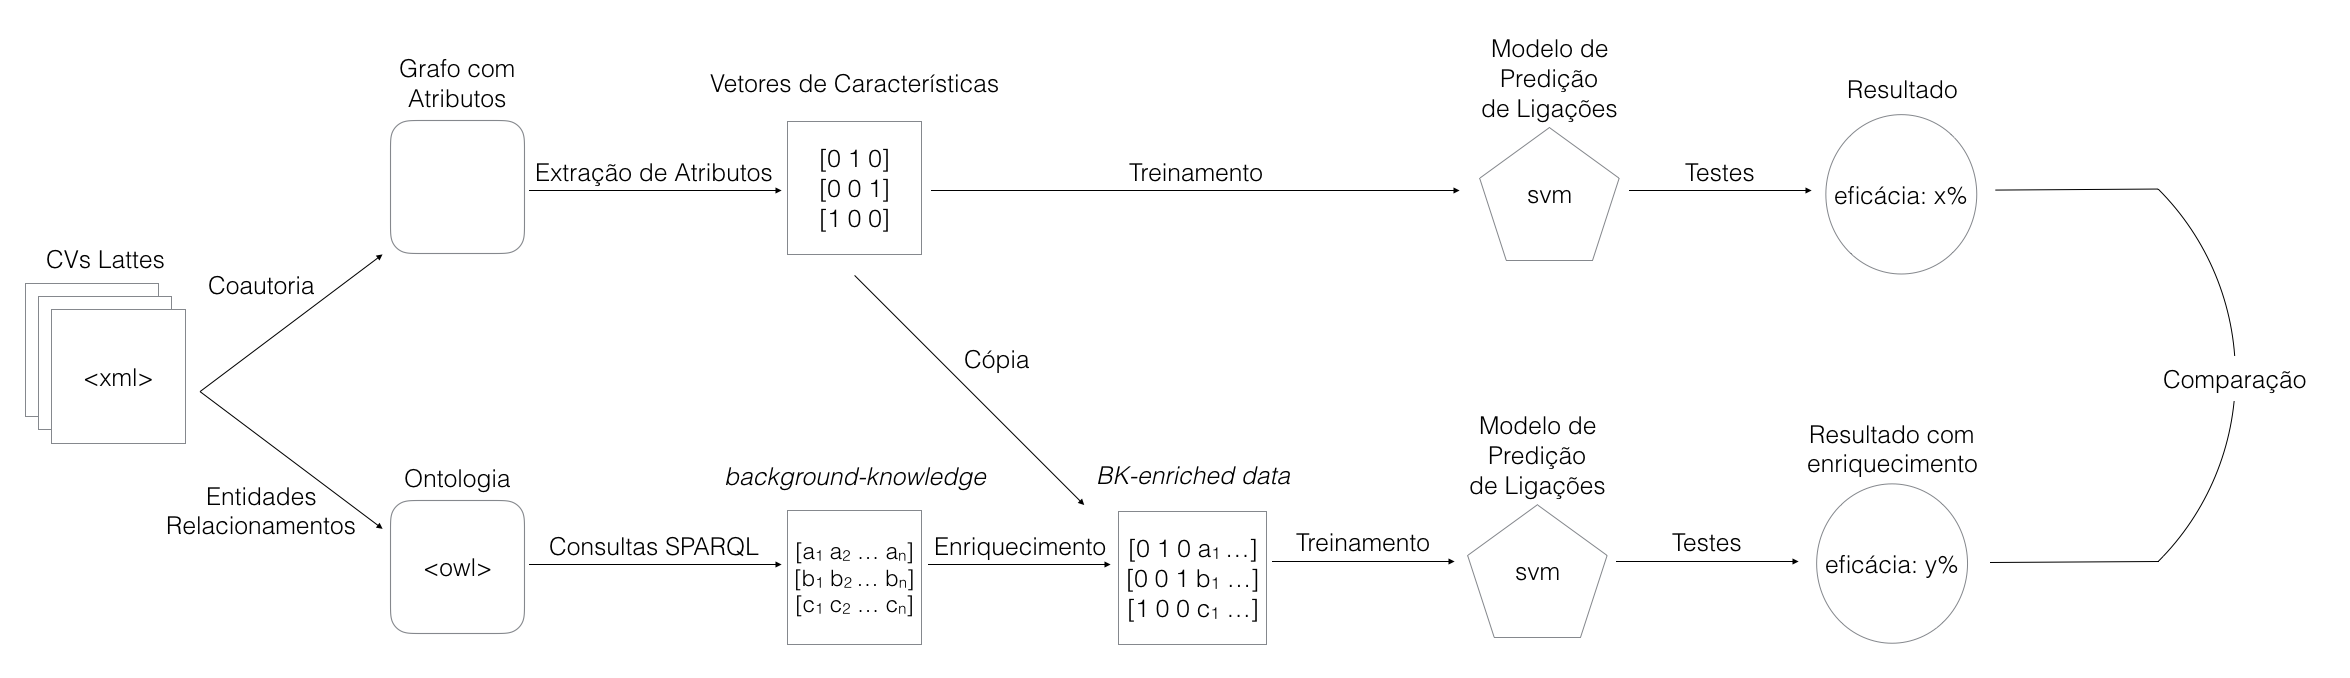
\includegraphics[width=.99\textwidth]{diagrama-menor}
  \caption{Diagrama de execução do experimento}
  \label{fig:diagrama-experimento}
\end{figure}

Ele está dividido em duas fases, a fase A e fase B. A fase A vai trabalhar apenas com dados relacionados à estrutura da rede, extraídos de um grafo. Já a B vai trabalhar com os dados sobre a estrutura da rede mais os dados extraídos da ontologia, que chamamos de conhecimento prévio. Os passos de cada fase serão discutidos a seguir.

Na fase A, um grupo pequeno de currículos lattes no formato XML será lido e processado, e serão extraídos dados gerais desses currículos. A partir desses dados, será construído um grafo com atributos, onde cada nó representa um pesquisador, e cada aresta representa alguma relação entre os participantes dessa rede.

Desse grafo, será extraído um conjunto de vetores de características, que chamamos de $VC$, separado em conjuntos de treinamento e teste. O modelo de predição será treinado com o conjunto de treinamento, e será testado com o conjunto de teste. Essa fase vai gerar um relatório que lista a eficácia do modelo, pois o resultado da classificação pode ser validado com os dados iniciais.

Na fase B, o mesmo grupo de currículos será processado, utilizando esses dados para popular a ontologia descrita anteriormente. Serão feitas consultas a respeito das entidades e relações presentes na ontologia e o seu resultado será transformado em um conjunto de atributos, denominado \textit{background-knowledge}, ou $BK$, como descrito anteriormente.

Os vetores de características ($VC$) da fase A serão copiados e associados ao conjunto $BK$, processo que chamaremos de enriquecimento com conhecimento prévio. Dessa forma, outro modelo de predição será instanciado e receberá como estrada esses dados enriquecidos, também separados em conjunto de treinamento e teste. Será feito o treinamento do modelo, depois o teste deste modelo, seguido de uma análise do resultado.

Por fim, será feita a comparação da eficácia de ambos os modelos, verificando se há alguma melhora no método. Também será avaliado se os atributos adicionais extraídos de $BK$ são relevantes para o modelo, através de uma análise da importância relativa de cada atributo na classificação final (\textit{feature selection}).

Em suma: o ambiente de testes recebe um conjunto de currículos e um arquivo OWL correspondente à estrutura da ontologia, porém sem nenhuma instância. O software faz o processamento (fases A e B), e gera ao final um relatório comparando ambas as estratégias.
